\newpage
\section{Evaluating Semantic `Goodness' of Machine Translated Texts}

Translation is becoming an utility in everyday life. The increased availability of real-time machine translation services relying on Statistical Machine Translation (SMT) allows users who do not understand the language of the source text to quickly gist text in a foreign language and understand its general meaning. For these users, often the accurate meaning of translated words is more important than the fluency of the translated sentence.

However, SMT can suffer from poor lexical choices. Fluent but inadequate translations are commonly produced due to the strong bias towards the language model component that prefers consecutive words based on the data that the system is trained on.

Current state of art MT evaluation metrics are generally able to identify problems with the grammaticality of the translation but less evidently the accuracy of translated semantics, e.g. incorrect translation of ambiguous words or wrong assignment of semantic roles. In the example below, the ideal Machine Translation (MT) evaluation metric should appropriately penalise poor lexical choice, such as `\textit{braked}', and reward or at least allow leeway for semantically similar translations, such as `\textit{external trade}'.

\begin{itemize}[noitemsep]
\item[] \textbf{Source (DE):} 
\item[] \textit{Auch der Aussenhandel bremste die Konjunktur.} 
\item[] \textbf{Phrase-based MT:} 
\item[] \textit{The foreign trade braked the economy.}
\item[] \textbf{Neural MT:} 
\item[] \textit{External trade also slowed the economy.}
\item[] \textbf{Reference (EN):} 
\item[] \textit{Foreign goods trade had slowed, too.}
\end{itemize}

The German word \textit{bremste} is commonly used as `\textit{braked}' in the context of driving, but the appropriate translation should have been `\textit{slowed}' in the example mentioned above. Although the phrase \textit{external trade} differs from f\textit{oreign goods trade} in the reference sentence, it should be considered as an acceptable translation.

To pursue a semantically motivated measure of goodness for machine translation, we pursue an evaluation metric that takes into account both fluency (grammaticality) and adequacy (semantics) to evaluate whether the machine translation output has the same meaning as its reference translation through the Semantic Textual Similarity (STS) task. Semantic Textual Similarity (STS) is the task of measuring the degree to which two texts have the same meaning \citep{Agirre2014}.  For instance, given the two texts,  ``\emph{the man is slicing the tape from the box.}" and ``\emph{a man is cutting open a box.}", an STS system predicts a real number similarity score on a scale of 0 (no relation) to 5 (semantic equivalence). In this case we can relate the pair of texts closely to what we are evaluating when measuring the goodness of machine translation output if we treat one of the sentence as the output and the other as the reference.

We propose a model that approaches the task by (i) combining existing machine translation evaluation metrics (that are good in determining fluency) and (ii) using linguistically motivated monolingual word alignments and neural embeddings (to add the semantic dimension to our new metric). We call our metric, {\tt Stasis}.\footnote{Part of the research in this chapter has been published in \cite{usaarsheff2015,usaarsheff2016}}

\subsection{Measuing Grammatical Fluency with MT Evaluation Metrics Ensemble}

Previous approaches have applied MT evaluation metrics for the STS task with progressively improving results \citep{Agirre2012,Agirre2013,Agirre2014,agirre2015}. We propose a single MT evaluation metric by ensembling a glut of MT evaluation metrics.\footnote{This section presents a collaborative work between Saarland University and University of Sheffield\footnote{A partner institute in the EXPERT project} in developing the MT evaluation metric ensemble.} 

\subsubsection{Previous Usage of MT Metrics to Determine Textual Similarity}
At the pilot English STS-2012 task, \cite{Rios2012} trained a Support Vector Regressor using the lexical overlaps between the surface strings, named entities and semantic role labels and the BLEU \citep{Papineni2002} and METEOR \citep{Banerjee2005,Denkowski2010} scores between the text snippets and their best system scored a Pearson correlation mean of 0.3825. The system underperformed compared to the organizers' baseline system\footnote{Refers to the token cosine baseline system ({\tt baseline-tokencos}) in STS-2012.} which scored 0.4356. 

For the English STS-2013 task, \cite{Barron-Cedeno2013} also used a Support Vector Regressor with an larger array of machine translation metrics (BLEU, METEOR, ROUGE \citep{lin-och:2004:ACL}, NIST \citep{doddington2002automatic}, TER \citep{snover2006study}) with measures that compute similarities of dependency and constituency parses \citep{liu2005syntactic} and semantic roles, discourse representation and explicit semantic analysis \citep{gabrilovich2007computing} annotations of the text snippets. These similarity measures are packaged in the Asiya toolkit \citep{Gimenez2010}. They scored 0.4037 mean score and performed better than the Takelab baseline \citep{vsaric2012takelab} at 0.3639.

At the SemEval-2014 Cross-level Semantic Similarity task \citep{jurgens2014crosssts,Jurgens2015}, participating teams submitted similarity scores for text of different granularity. \cite{Huang2014} used a linear regressor solely with MT evaluation metrics (BLEU, METEOR, ROUGE) to compute the similarity scores between  paragraphs and sentences. They scored 0.792 beating the lowest common substring baseline which scored 0.613.

In the SemEval-2015 English STS and Twitter similarity tasks, \citep{berterofung2015} trained a neural network classifier using (i) lexical similarity features based on WordNet \citep{miller1995wordnet}, (ii) neural auto-encoders \citep{socher2011dynamic}, syntactic features based on parse tree edit distance \citep{zhang1989simple,wan2006using} and (iii) MT evaluation metrics, viz. BLEU, TER, SEPIA \citep{habash2008sepia}, BADGER \citep{parker2008badger} and MEANT \citep{lo2012fully}.

For the classic English STS task in SemEval-2015, \cite{usaarsheff2015} used a range of MT evaluation metrics based on lexical (surface $n$-gram overlaps), syntactic (shallow parsing similarity) and semantic features (METEOR variants) to train a Bayesian ridge regressor. Their best system achieved 0.7275 mean Pearson correlation outperforming the {\tt token-cos} baseline which scored 0.5871 while the top system \citep{sultan2015} achieved 0.8015.

Another notable mention of MT technology in the STS tasks is the use of referential translation machines to predict and derive features instead of using MT evaluation metrics \citep{Bicici2013,Bicici2014,bicici2015}.

\subsubsection{Feature Matrix}

Following the success of STS systems that use MT evaluation metrics, we train three regression models using an array of MT metrics based on lexical, syntactic and semantic features. 

Machine translation evaluation metrics utilize various degrees of lexical, syntactic and semantic information. Each metric considers several features that compute the translation quality by comparing a translation against one or several reference translations. 

We trained our system using the follow feature sets: (i) $n$-gram, shallow parsing and named entity overlaps ({\tt Asiya}), (ii) {\tt BEER}, (iii) {\tt METEOR} and (iv) {\tt ReVal}. Although {\tt BEER} and {\tt METEOR} metrics provided mecahnisms to fine-tuned the metric with respect to the training data, we did not tune these metrics because they will be used as input features that will be fed into an ensemble which will automatically learn their feature weights which effectively fine-tuned the metric to the training data too. 

\textbf{{\tt Asiya} Features}: \cite{gonzalez2014} introduced a range of language independent metrics relying on $n$-gram overlaps similar to the modified $n-$-gram precisions of the BLEU metric \citep{Papineni2002}. Different from BLEU, \cite{gonzalez2014} computes $n$-gram overlaps using similarity coefficients instead of proportions. We use the {\tt Asiya} toolkit \citep{Gimenez2010} to annotate the dataset with the similarity coefficients of $n$-gram overlap features described in this section. We use 16 features from both cosine similarity and Jaccard Index coefficients of the character-level and token-level $n$-grams from the order of bigrams to 5-grams. Additionally, we use the Jaccard similarity of the pseudo-cognates and the ratio of $n$-gram length as the 17th and 18th features. Adding a syntactic dimension to our feature set, we use 52 shallow parsing features described in \cite{usaarsheff2015}; they measure the similarity coefficients from the $n$-gram overlaps of the lexicalized shallow parsing (aka chunking) annotations. As for semantics, we use 44 similarity coefficients from Named Entity (NE) annotation overlaps between two texts. After some feature analysis, we found that 22 out of the 44 NE $n$-gram overlap features and 1 of the shallow parsing features have extremely low variance across all sentence pairs in the training data. We removed these features before training our models.

\textbf{{\tt BEER} Features}: \cite{stanojevic2014beer} presents an MT evaluation metric that uses character $n$-gram overlaps, the Kendall tau distance of the monotonic word order \citep{isozaki2010automatic,birch2010lrscore} and abstract ordering patterns from tree factorization of permutations \citep{zhang2007factorization}. While Asiya features are agnostic to word classes, BEER differentiates between function words and non-function words when calculating its adequacy features. 

\textbf{{\tt METEOR} Features}: METEOR first aligns the translation to its reference, then it uses the unigram mapping to see whether they match based on their surface forms, word stems, synonyms and paraphrases \citep{Banerjee2005,Denkowski2010}. Similar to BEER features, METEOR makes a distinction between content words and function words and its recall mechanism weights them differently. We use all four variants of METEOR: exact, stem, synonym and paraphrase. 

\textbf{{\tt ReVal} Features}: ReVal \citep{reval2015} is a deep neural net based metric which uses the cosine similarity score between the Tree-based Long Short Term Memory (LSTM) \citep{hochreiter1997long,cho2014,treelstm} dense vector space representations of two sentences.

\subsubsection{The MT Metric Ensemble}

The STS 2012 to 2015 datasets are made up of sentence pairs with manually annotated scores of the similarity between each pair of sentences. We annotated the STS 2012 to 2015 datasets with the features as described in the previous section and trained three models using (i) a linear regressor ({\tt Linear}), (ii) boosted tree regressor ({\tt Boosted}) \citep{friedman2001greedy} and (iii) eXtreme Gradient Boosted tree regressor ({\tt XGBoost}) \citep{chen2015xgboost,chenxgboost}.

%%%%%%%%%%%%%%%%%%%%%%%%%%%%%%%%%%%%%%%%%%%%%%%%%%%%%%%%%%%%%%%%%%

\subsection{Measuing Semantic Adequacy With Monolingual Word Alignments and Neural Network Embeddings}

For the 2014 and 2015 editions of the STS task, the top performing submissions are from the DLS@CU team \citep{sultan2014dls,sultan2015dls}. 

Their STS2014 submission is based on the proportion of overlapping content words between the two sentences treating semantic similarity as a monotonically increasing function of the degree to which two sentences contain semantically similar units and these units occur in similar semantic contexts \citep{sultan2014dls}. Essentially, their semantic metric is based on the proportion of aligned content words between two sentences, formally defined as:

\vspace{-2mm}

\begin{equation}\label{eq:prop-al}
{ prop }_{ Al }^{ (1) }=\frac { |\{ i:[\exists j:(i,j)\in Al] \ and \ { w }_{ i }^{ (1) }\in C\} | }{ |\{ i:{ w }_{ i }^{ (1) }\in C\} | } 
\end{equation}

where ${ prop }_{ Al }^{ (1) }$ is the monotonic proportion of the semantic unit alignment from a set of alignments $Al$ that maps the positions of the words $(i,j)$ between sentences $S^{(1)}$ and $S^{(2)}$, given that the aligned units belong to a set of content words, $C$. Since the proportion is monotonic, the equation above only provides the proportion of semantic unit alignments for $S^{(1)}$. The $Al$ alignments pairs are automatically annotated by a monolingual word aligner \citep{sultan2014back} that uses word similarity measures based on contextual evidence from the Paraphrase Database (PPDB) \citep{ppdb} and syntactic dependencies.

The same computation needs to be made for $S^{(2)}$. An easier formulation of Equation \eqref{eq:prop-al} without the formal logic symbols is:

\vspace{-5mm}

\begin{equation}\label{eq:prop-al-pythonic}
{ prop }_{ Al }^{ (1) }=\frac { sum(1 \ for \ { w }_{ i },{ w }_{ j } \ in \ { Al }^{ (1,2) } \ if \ { w }_{ i } \ in \ C) }{ sum(1 \ for \ { w }_{ i } \ in \ { S }^{ (1) } \ if \ { w }_{ i } \ in \ C) } 
\end{equation}

\vspace{2mm}

Since the semantic similarity between  $(S^{(1)}, S^{(2)})$ should be a single real number, \cite{sultan2014dls} combined the proportions using harmonic mean:

\vspace{-5mm}

\begin{equation}\label{eq:sim-sent}
sim({ S }_{  }^{ (1) },{ S }_{  }^{ (2) })=\frac { 2*{ prop }_{ Al }^{ (1) }*{ prop }_{ Al }^{ (2) } }{ { prop }_{ Al }^{ (1) }+{ prop }_{ Al }^{ (2) } } 
\end{equation}

Instead of simply using the alignment proportions, \cite{sultan2015dls} extended their hypothesis by leveraging pre-trained neural net embeddings \citep{baroni2014composes}. \cite{sultan2015dls}  posited that the semantics of the sentence can be captured by the centroid of its content words\footnote{In the implementation, they have used lemmas instead of words to reduce sparsity when looking up the pre-trained embeddings (personal communication with Arafat Sultan).} computed by the element-wise sum of the content word embeddings normalized by the number of content words in the sentence. Together with the similarity scores from Equation \eqref{eq:sim-sent} and the cosine similarity between two sentence embeddings, \cite{sultan2015dls} trained a Bayesian ridge regressor to learn the similarity scores between text snippets. 

\subsubsection{Replicating of DLS}

To replicate the success of \cite{sultan2014dls}, we use the monolingual word aligner from \cite{sultan2014back} to annotate the STS-2012 to STS-2015 datasets and computed the alignment proportions as in Equation \eqref{eq:prop-al} and \eqref{eq:prop-al-pythonic}.

In duplicating \cite{sultan2015dls} work, we first have to tokenize and lemmatize text. The details of pre-processing choices was undocumented in their paper, thus we lemmatized the datasets with the NLTK tokenizer \citep{bird2009natural} and PyWSD lemmatizer \citep{pywsd14}. We use the lemmas to retrieve the word embeddings from the COMPOSES vector space \citep{baroni2014composes}. Similar to Equation \eqref{eq:prop-al-pythonic} (changing only the numerator), we sum the sentence embedding's centroid as follows:

\vspace{-5mm}

\begin{equation}
v(S_{  }^{ (1) })=\frac { sum(v({ w }_{ i }) \ for \ { w }_{ i } \ in  \ { S }^{ (1) } \  if \ { w }_{ i } \ in  \ C) }{ sum(1 \ for \ { w }_{ i } \ in \ { S }^{ (1) } \ if \ { w }_{ i } \ in \ C) } 
\end{equation}

where $v(S_{  }^{ (1) })$ refers to the dense vector space representation of the sentence $S_{  }^{ (1) }$ and $v({ w }_{ i })$ refers to the word embedding of word $i$ provided by the COMPOSES vector space. The same computation has to be done for $S_{  }^{ (2) }$.

Intuitively, if either of the sentences contains more or less content words than the other, we can see the numerator changing but the denominator changes with it. The difference between $v(S_{  }^{ (1) })$ and $v(S_{  }^{ (2) })$ contributes to \emph{distributional semantic distance}. 

To calculate a real value similarity score between the sentence vectors, we take the dot product between the vectors to compute the cosine similarity between the sentence vectors:

\vspace{-2mm}

\begin{equation}
sim({ S }_{  }^{ (1) },{ S }_{  }^{ (2) })=\frac { v(S_{  }^{ (1) })\cdot v(S_{  }^{ (2) }) }{ |v(S_{  }^{ (1) })| \ |v(S_{  }^{ (2) })|  } 
\end{equation}

There was no clear indication of which vector space \cite{sultan2015dls} have chosen to compute the similarity score from Equation 5.5. Thus we compute two similarity scores using both COMPOSES vector spaces trained with these configurations:

\begin{itemize}
\item 5-word context window, 10 negative samples, subsampling, 400 dimensions
\item 2-word context window, PMI weighting, no compression, 300K dimensions
\end{itemize}

In this way, we extracted two similarity features for every sentence pair. With the harmonic proportion feature from Equation 5.3 and the similarity scores from Equation 5.5, we trained a boosted tree ensemble on the 3 features using the STS 2012 to 2015 datasets and submitted the outputs from this model as our baseline submission in the English STS Task in SemEval 2016. 

\subsubsection{Replacing COMPOSES with GloVe}

\cite{glove2014} handles semantic regularities \citep{levy2014linguistic} explicitly  by using a global log-bilinear regression model which combines the global matrix factorization and the local context vectors when training word embeddings.

Instead of using the COMPOSES vector space, we experimented with replacing the  $v({ w }_{ i })$ component in Equation 5.4 with the GloVe vectors,\footnote{We use the 300 dimensions vectors from the GloVe model trained on the Commoncrawl Corpus with 840B tokens, 2.2M vocabulary.} $v_{glove}({ w }_{ i })$ such that:

\vspace{-5mm}

\begin{equation}
sim_{glove}({ S }_{  }^{ (1) },{ S }_{  }^{ (2) })=\frac { v_{glove}(S_{  }^{ (1) })\cdot v_{glove}(S_{  }^{ (2) }) }{ |v_{glove}(S_{  }^{ (1) })| \ |v_{glove}(S_{  }^{ (2) })|  } 
\end{equation}

\vspace{2mm}

The novelty lies in the usage of the global matrix to capture corpus wide phenomena that might not be captured by the local context window. The model leverages on both the non-zero elements in the word-word co-occurence matrix (not a sparse bag-of-words matrix) and the individual context window vectors similar to the word2vec model \citep{mikolov2013distributed}. 

\subsubsection{Similarity Using Tree LSTM}
Recurrent Neural Nets (RNNs) allow arbitrarily sized sentence lengths \citep{elman1990finding} but early work on RNNs suffered from the vanishing/exploding gradients problem \citep{bengio1994learning}. \cite{hochreiter1997long} introduced multiplicative input and output gate units to solve the vanishing gradients problem. While RNN and LSTM process sentences in a sequential manner, Tree-LSTM extends the LSTM architecture by processing the input sentence through a syntactic structure of the sentence. We use the ReVal metric \citep{reval2015} implementation of Tree-LSTM \citep{tai-socher-manning:2015}  to generate the similarity score.

ReVal represents both sentences ($h_{1}$, $h_{2}$) using Tree-LSTMs and predicts a similarity score $\hat{y}$ based on a neural network which considers both distance and angle between $h_{1}$ and $h_{2}$:

\begin{equation}
%\begin{align}
\label{eq2}
\begin{split}
h_{\times} & =h_{1}\odot h_{2}
\\ 
h_+ & =|h_{1}-h_{2}| 
\\
h_s & =\sigma\left(W^{(\times)}h_{\times} + W^{(+)}h_+ +b^{(h)}\right)
\\
\hat{p}_{\theta} & = \text{softmax} \left(W^{(p)}h_s + b^{(p)}\right)
\\
\hat{y} & =r^T\hat{p}_{\theta}
\end{split}
%\end{align}
\end{equation}
where, $\sigma$ is a sigmoid function, $\hat{p}_\theta$ is the estimated probability distribution vector and $r^T=[1$ $2 ... K]$. 
The cost function $J(\theta)$ is defined over probability distributions $p$ and $\hat{p}_{\theta}$  using regularised Kullback–Leibler (KL) divergence. 
\begin{equation}
\label{eq3}
J(\theta)  = \frac{1}{n} \sum_{i=1}^{n} \text{KL}\left(p^{(i)}\middle|\middle|\hat{p}_{\theta}^{(i)}\right) + \frac{\lambda}{2}{||\theta||}_2^2
\end{equation}
In Equation \ref{eq3}, $i$ represents the index of each training pair, $n$ is the number of training pairs and $p$ is the sparse target distribution such that $y=r^Tp$ is defined as follows:
\[
    p_j= 
\begin{cases}
    y- \lfloor{y\rfloor},& j = \lfloor{y\rfloor} + 1\\
    \lfloor{y\rfloor} -y +1, & j = \lfloor{y\rfloor}\\
    0              & \text{otherwise}
\end{cases}
\]
for $1\le j \le K$, where, $y\in[1, K]$ is the similarity score of a training pair. This gives us a similarity score between [1, K] which is mapped to [0, 1].\footnote{score = (score-1)/K Please refer to \cite{reval2015} for training details.}

\subsubsection{A Semantically Adequate Metric}

Similar to our approach in the MT metric ensemble, we annotated the STS 2012 to 2015 datasets with the semantic similarity features as described in the previous section and trained three models using (i) a linear ridge regressor ({\tt L}) that uses the similarity score from Equations 6.3 and 6.5 as features, (ii) extending the linear regression, we included the similarity score from Equations 6.6 and 6.8 to the feature set and trained a boosted tree ensemble \citep{friedman2001greedy} ({\tt B}) (iii) we use the same feature set as our B system to train an eXtreme Gradient Boosted tree regressor ({\tt XGBoost}) \citep{chen2015xgboost,chenxgboost}, we refer to it as ({\tt X}).

\subsection{Experimental Setup and Results}

We evaluated the two components of our {\tt Stasis} metric using the STS2016 dataset that consist of text snippets from the following domains, (i) forum answers, (ii) forum questions, (iii) news headlines, (iv) plagiarism checking samples from student essays and (v) post-editing texts.

\begin{table}[H]
\centering
    \begin{tabular}{l|ccccc|c}
            & answer-answer & headlines & plagiarism & postediting & question-question & Overall     \\ \hline
    {\tt MT Ensemble (L)}  & 0.31539       & 0.76551   & 0.82063    & 0.83329     & \textbf{0.73987}           & 0.68923 \\
    {\tt MT Ensemble (B)} & 0.37717       & 0.77183   & 0.81529    & 0.84528     & 0.66825           & 0.69259 \\
    {\tt MT Ensemble (X)} & \textit{0.47716} & \textbf{0.78848} & \textbf{0.83212}    & \textit{0.84960}      & 0.69815           & \textit{0.72693} \\ \hline
   {\tt Semantic (L)} & 0.48799       & 0.71043   & 0.80605    & 0.84601     & 0.61515           & 0.69244 \\
    {\tt Semantic (B)}  & 0.49415       & 0.71439   &\textit{ 0.79655 }   & 0.83758     & \textit{0.63509 }          & 0.69453 \\
    {\tt Semantic (X)}  & \textit{0.49947 }      & \textit{0.72410 }   & 0.79076    & \textit{0.84093}     & 0.62055           & \textit{0.69471} \\ \hline
\textbf{{\tt Stasis (X)}} & \textbf{0.50628} &  0.77824 & 0.82501 &  \textbf{0.84861} & 0.70424 & \textbf{0.73050} \\ \hline
Median & 0.48018 & 0.76439 & 0.78949 & 0.81241 & 0.57140 & 0.68923 \\
Best & 0.69235 & 0.82749 & 0.84138 & 0.86690 & 0.74705 & 0.77807 \\
    \end{tabular}
\caption{{\tt Stasis} Metric Evaluated on the STS-2016 Task;  \textit{Best} is the best performing results per domain from various systems participating in the English STS-2016 shared task and \textit{Median} is the median scores from all participating systems in the English STS-2016 shared task.}
\label{tab:sts1}
\end{table}

Table \ref{tab:sts1} presents the results for evaluating our {\tt Stasis} metric on the English STS-2016 dataset. 
The top part of the table presents the results of the component that ensembles the MT evaluations metrics and the second portion of the table presents the results of the semantic adequacy component that uses linguistically motivated monolingual word alignment and neural network embeddings. The bottom-most part of the table presents the median and the best correlation results across all participating teams in the STS-2016 task.

Our MT metric ensemble system, our baseline linear model outperforms the median scores for all domains except the \emph{answer-answer} domain. Our boosted tree model performs better than the linear model and the extreme gradient boosted tree model performs the best of the three. We note that our correlation scores for all three models is lower than the median for the \emph{answer-answer} domain. 

As for our semantic adequacy component, the median and best scores are computed across all participating teams in the task. Our baseline system performs reasonably well, outperforming the median scores in most domains. Our extended variant of the baseline using boosted tree ensemble performs better in the answer-answer, headlines and postediting domains but performed worse in others. Comparatively, it improves the overall correlation score marginally by 0.002. The system using XGBoost performs the best of the 3 models but it underperforms in the headlines and plagiarism domain when compared to the median scores. 

When the MT evaluation ensemble and the semantic adequacy is combined using the XGBoost regressor, we achieved a higher score for every domain leading to an overall Pearson correlation score of 0.73050 ({\tt Stasis (X)} in Table \ref{tab:sts1}).

\subsubsection{Inadequacy in Current MT Evaluation Metrics}

In this section, we look closer at the inadequacy of the MT metric ensemble system. Figure \ref{fig:sts1} shows the bubble chart of the L1 error analysis of our XGBoost model against the gold standard similarity scores for the answer-answer domain. The colored lines correspond to the integer annotations, e.g. the yellow line represents the data points where the gold-standard annotations are 1.0. The span of the line represents the span of predictions our model made for these texts. The size of the bubble represents the effect size of our predictions' contribution to the Pearson correlation score, i.e. how close our predictions are to the gold standards.

\begin{figure}[!htb]
    \centering
    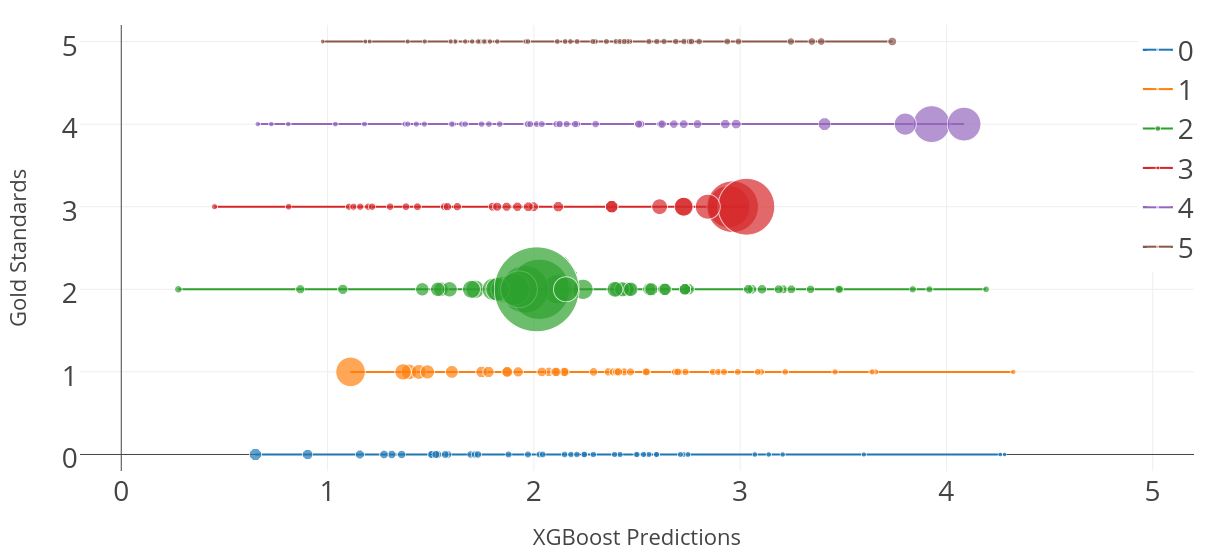
\includegraphics[width=0.92\textwidth]{images/saar-sheff-ans-ans}
    \caption{L1 Error Analysis on the answer-answer domain}
    \label{fig:sts1}
\end{figure}

\begin{figure}[!htb]
    \centering
    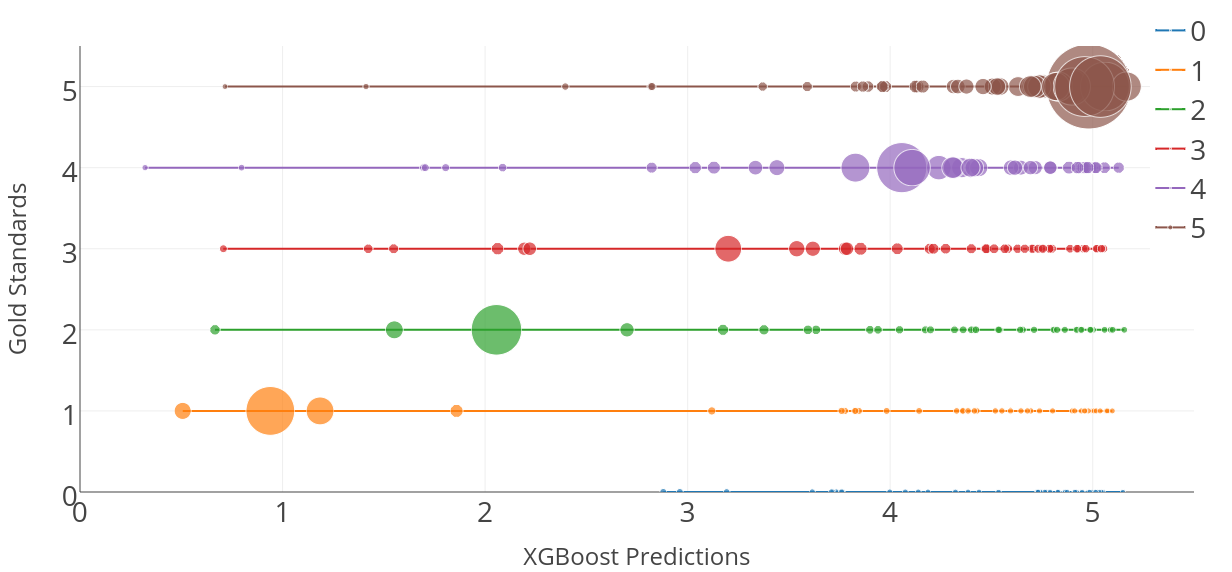
\includegraphics[width=0.92\textwidth]{images/saar-sheff-postediting}
    \caption{L1 Error Analysis on the post-editing domain}
    \label{fig:sts2}
\end{figure}

As we see from Figure \ref{fig:sts1}, the centroids of the bubbles represents our model's best predictions. Our predictions for texts that are annotated at 1 to 4 similarity scores are reasonably close to the gold standards but the model performs poorly for texts annotated with the 0 and 5 similarity scores. 

Looking at the texts that are rated 0, we see that there are cases where the $n$-grams within these texts are lexically / syntactically similar but the meaning of the texts are disparate. For example, this pair of text snippets, \emph{`You don't have to know'} and \emph{`You don't have equipments/facilities'} are rated 0 in the gold standards but from a machine translation perspective, a translator would have to do little work to change \emph{`to know'} to \emph{`equipments/facilities'}. 

Because of this, machine translation metrics would rate the texts as being similar and even suitable for post-editing. However, the STS task focuses only on the meaning of the text which corresponds more to the adequacy aspect of the machine translation metrics. Semantic adequacy is often overlooked in machine translation because our mass reliance on BLEU scores to measure the goodness of translation with little considerations for penalizing semantic divergence between the translation and its reference.

On the other end of the spectrum, machine translation metrics remain skeptical when text snippets are annotated with a score of 5 for being semantically analogous but syntactically the texts are expressed in a different form. For example, given the text snippets, \emph{`There's not a lot you can do about that'} and \emph{`I'm afraid there's not really a lot you can do'}, most machine translation metrics will not allocate full similarity scores due to the difference in lexical and stylistic ways in which the sentences are expressed. 

Machine translation metrics' failure to capture similarity score extremes is evident in Figure \ref{fig:sts1} where there are no 0 and 5.0 predictions. 

Naturally the XGBoost predictions based on the MT evaluation metric features fit the postediting domain. Figure \ref{fig:sts2} shows that the centroids in the L1 Figure for the postediting domain is more centered than in the answer-answer domain.

\subsection{Summary}

In this section, we pursue a combination machine translation evaluation metric {\tt Stasis} to evaluate the grammaticality and semantic adequacy between pairs of sentences. We combined existing machine translation evaluation metrics (that are good in determining fluency) and used linguistically motivated monolingual word alignments and neural embeddings to add the semantic dimension to our new metric.